% !TEX root = Master.tex

The next step, after fitting proper models to the marginal distributions of the log-sales aggregated on key category cluster level, is to enter the pairwise modelling of the clusters. Specifically, we are interested in capturing the dependence structure over time which is delineated in the next three Subsections (\ref{sssec:kcc_26}, \ref{sssec:kcc_28} and \ref{sssec:kcc_68}).
\\

Recalling the previous Section \ref{ssec:kcc_marginals}, the residuals from the fitting method are depicted in \autoref{fig:res_gamlss_over_time} for each time-point. In a second step, the residuals will be used in a pairwise fashion after the marginal modelling to estimate the dependence structure with the help of conditional copulas (see Section \ref{ssec:conditional_copulas}).

\begin{figure}[H]
\centering
  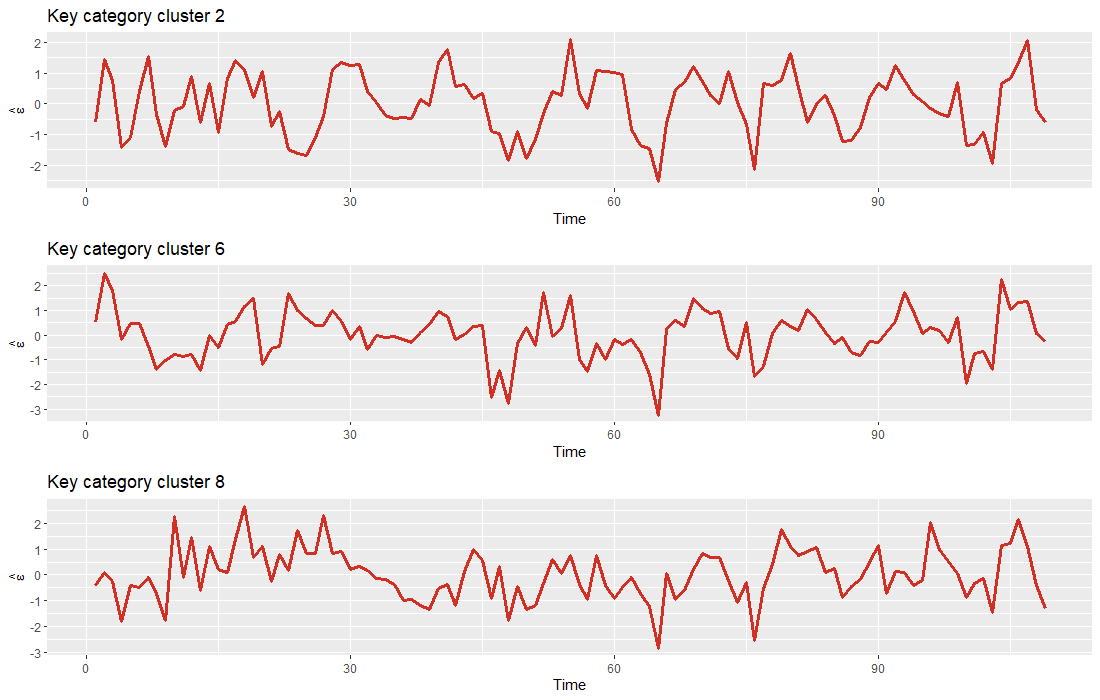
\includegraphics[width=0.95\linewidth]{figures/res_gamlss_over_time.png}
  \caption{Estimated residuals of GAMLSS fits for the three key category clusters}
  \label{fig:res_gamlss_over_time}
\end{figure}






\inputRoutput[caption={AIC values of distribution fits on KCC with \textit{fitDist()} function of the \textit{gamlss} package},numbers=left,numberstyle=\tiny, label=output:gamlss_distributions_aic]{gamlss_distributions_aic.txt}



In the previous Section \ref{ssec:kcc_marginals}, the model fits resulted in quantile residuals that we were able to approximate parametrically by normal distributions. When the three sets of residuals are passed into the \textit{fitDist()} function of the \textit{gamlss} package, it returns multiple suggestions of parametric distribution that can be used to fit to the data, ordered by ascending \ac{AIC}. An excerpt is given in R output \ref{output:gamlss_distributions_aic}. The only distributions that are also at the disposal of the \textit{gjrm} package\footnote{Elaboration on this in the following subsections.} are the normal and the logistic distributions and the \ac{AIC} values are close, indicating that both are good fits. Thus, the normal distribution is chosen for all three residual sets in the following.


